%! Author = lili
%! Date = 6/9/26

% 169-172: Die hnRNA reift im Zellkern zur mRNA - Mosaikgene
% 215-218: Regulation der Genaktivität bei Prokaryonten - Regulation des X-Phagen; Regulation der Genaktivität bei Eukaryonten
% 221: Regulation der Genaktivität bei Eukaryonten - Regulation der Transkription durch Chromatinproteine
% 227-231: Regulation der Genaktivität bei Eukaryonten - Kontrolle der Transkription durch Promotoren und Enhancer;
% Verwendung unterschiedlicher Promotoren; Regulatorische DNA-Elemente kontrollieren gewebe- und
%zeitspezifische Transkription; Posttranskriptionelle Regulation der Genexpression; Regulation durch Alternatives Spleißen

% bis F 18 wdh

Folie 15 bis
entspricht v4 aus Eukgen\ldots daraus kopieren, wenn fertig.

zusätzlich:


\subsubsection*{Typische Promotoren}
% TODO F 19

\defin{operon}

% TODO Bild F 20

\defin{rbs}
% TODO mehr dazu
\defin{polycistronisch}
\defin{monocistronisch}

\begin{figure}[H]
    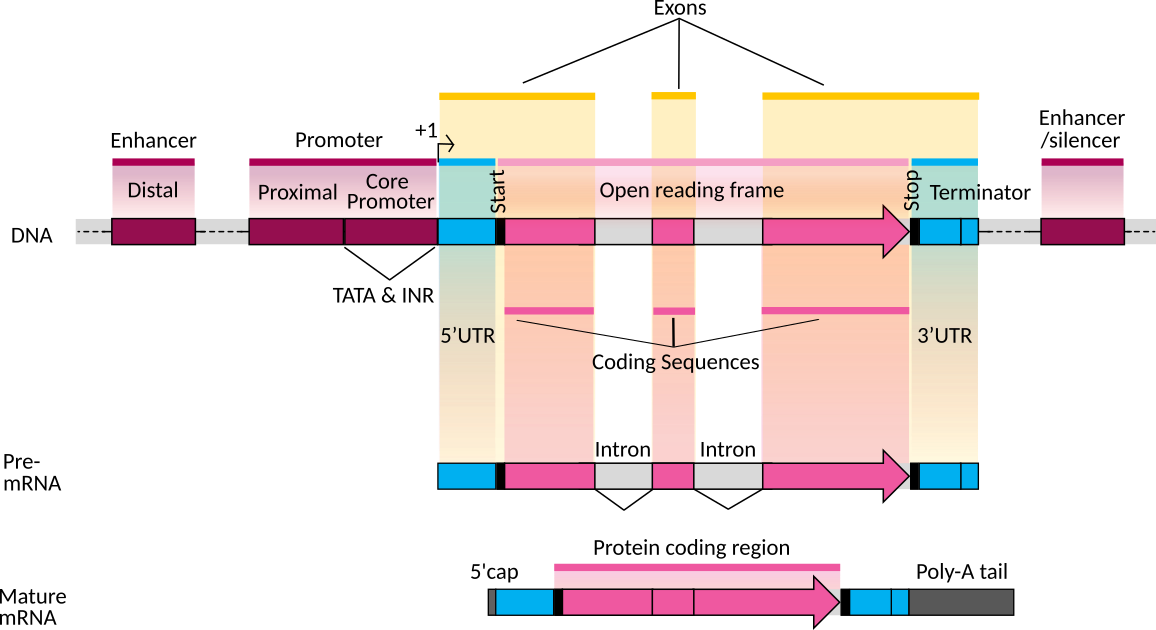
\includegraphics[width=\textwidth]{../eukgen/images/eukgen}
    \caption{Pol II.}\label{fig:figure25}
\end{figure}

\defin{inr}

% Core promotor etc Eukgen 36

% BOXEN

\defin{ciselement}
\defin{transelement}

% Transkriptionsfaktoren
% TODO schauen ob rtf und gtf defis haben
% TODO F 31

\defin{dbd}

\defin{bzip}
\defin{bhlh}
\defin{myb}

% TODO F 31 - 34 #

% evtl. TODO F 35 - 36

% TODO Präinitiationskomplex F 37

% TODO Transkription F 38 - 43

% TODO interrupted genes F 44

\section{Spleißen}\label{sec:spleien}
% TODO F 45 - 51
% TODO Trans-Esterifizierung

% TODO Zusammenfassung mRNA-Bildung F 52 hier UND in eukgen!


\subsection{Aufbau der eukaryotischen \gls{mrna}}\label{subsec:aufbau-der-eukaryotischen-gls{mrna}}
% TODO Frage Was muss man über die Enden der euk \gls{mrna} wissen
Die Enden eukaryotischer \gls{mrna} sind modifiziert, was sie von prokaryotischer \gls{mrna} unterscheidet.
Eukaryotische \gls{mrna} besitzt am 5'-Ende eine Cap-Struktur und am 3'-Ende einen \gls{polya}.
Beide schützen die \gls{mrna} vor Abbau und fördern ihre Translation.

\begin{figure}[H]
    \centering
    % TODO Bilderverdeckung
    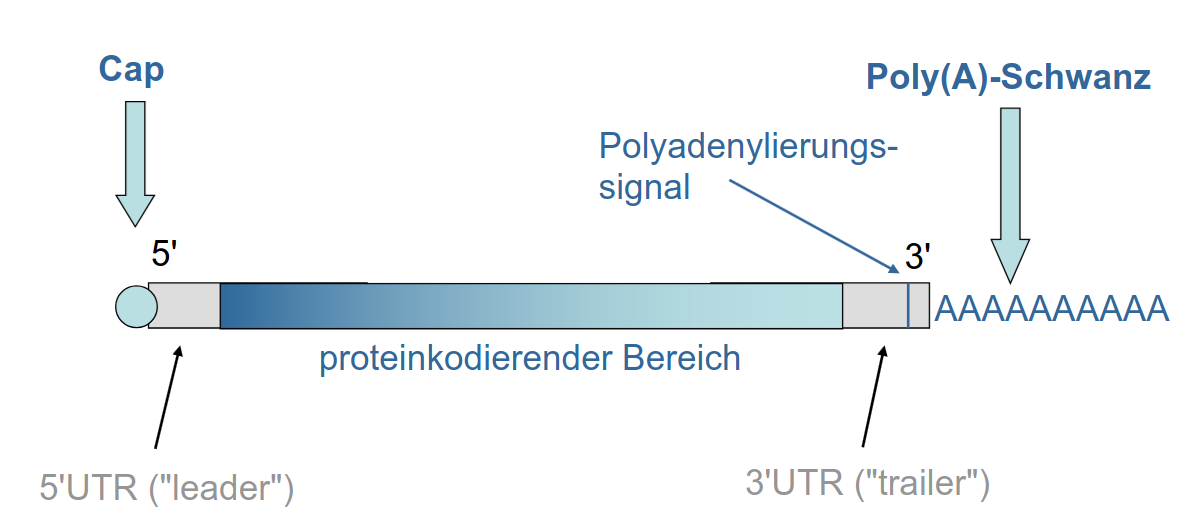
\includegraphics[width=0.7\linewidth]{../eukgen/images/euk_rna}
    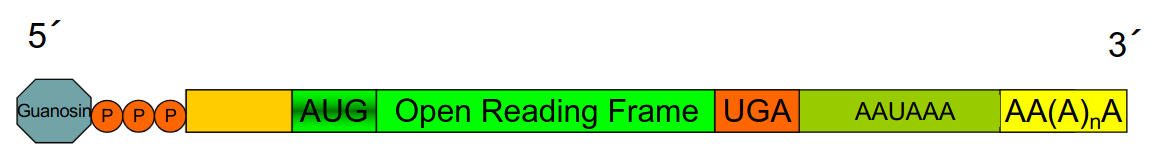
\includegraphics[width=0.7\linewidth]{../eukgen/images/euk_rna_2}
    \caption{Bilder aus Vorlesungsfolien}\label{fig:figure5}
\end{figure}

\defin{cap}
\defin{leader}
\defin{trailer}
\defin{pas}
\begin{table}[ht]
    \centering
    \renewcommand{\arraystretch}{1.3}
    \begin{tabular}{|l|p{10cm}|}
        \textbf{\gls{mrna}-Teil} & \textbf{Funktion} \\
        5'-\gls{cap}; GTP & Schutz der \gls{mrna} vor Abbau, Bindung des Ribosoms \\
        \gls{leader} & Binden des Ribosoms \\
        AUG & Startcodon, Beginn der Translation mit Methionin \\
        \gls{orf} & Der \gls{orf} codiert die Abfolge der Aminosäuren \\
        UGA & Stopcodon für das es keine beladene \gls{trna} gibt \\
        \gls{trailer} mit (AAUAAA) & Signal zum Schneiden und die Polyadenylierung \\
        \gls{polya} & Stabilisierung der \gls{mrna} \\
    \end{tabular}
    \caption{Funktionelle Elemente der eukaryotischen \gls{mrna}}
    \label{tab:mrna}
\end{table}


\section{Transport der mRNA aus dem Zellkern}\label{sec:transport-der-mrna-aus-dem-zellkern}

\subsection{rDNA}\label{subsec:rdna}
\defin{rdna}
Die Ribosomen von Eukaryonten werden im \gls{nukleolus} zusammengebaut.
Die Bildung des \gls{nukleolus} geht vom Nukleolus‐Organisator, der aus der \gls{nor} entsteht. %\cite{Knust2025_Meiose}


Besonderheit der \gls{rdna}: Sie hat eine ``Sichtbare Genexpression''.
D.h.\ man die Genexpression direkt ``sehen'',
weil das Genprodukt selbst \gls{rna} ist.

% TODO F 59

\section{Kompartimentierung der Zelle}\label{sec:kompartimentierung-der-zelle}
Spezifische Funktionen erfordern eine Ausstattung mit
spezifischen Proteinen und die Kompartimentierung der Zelle
schafft spezialisierte Funktionsräume. \cite{vorlesung13}

\subsection{Die Orte der Proteinbiosynthese}\label{subsec:die-orte-der-proteinbiosynthese}
\begin{mytable}
    \begin{tabular}{c|c}
        \textbf{Lokalisierung der Ribosomen} & \textbf{Art der synthetisierten Proteine} \\

        Mitochondrium
        & Proteine, die durch die mitochondriale DNA kodiert werden \\


        Chloroplasten
        & Proteine, die durch die Chloroplasten-DNA kodiert werden \\


        Cytosolische Ribosomen
        & Cytosolische-, Mitochondrien-, Chloroplasten-, Peroxisomen- und Zellkern-Proteine \\


        ER-gebundene Ribosomen
        & Membranproteine der Plasma-, Kern-, ER-, Golgi-, Lysosomen- und Endosomenmembran; sekretierte Proteine \\

    \end{tabular}
    \caption{Zusammenhang zwischen Ribosomenlokalisierung und synthetisierten Proteinen}
\end{mytable}
Als Fließtext: \\
Ribosomen unterscheiden sich je nach ihrem Ort in der Zelle darin, welche Proteine sie herstellen.
Ribosomen in Mitochondrien und Chloroplasten produzieren Proteine, die von der jeweiligen Organellen-DNA codiert werden.
Cytosolische Ribosomen stellen dagegen Proteine für das Cytosol sowie für Mitochondrien, Chloroplasten, Peroxisomen und den Zellkern her.
An das endoplasmatische Retikulum (ER) gebundene Ribosomen produzieren vor allem Membranproteine für Zellmembranen (z.
B. Plasma-, Kern-, ER-, Golgi-, Lysosomen- und Endosomenmembranen) sowie Proteine, die aus der Zelle ausgeschleust werden.

% TODO aus Eukgen V8
TODO aus Eukgen V8
% TODO F 63 Bild
% TODO F 64 - 66 und schauen, ob davon noch was in Eukgen kann

% TODO Ebenen der Genregulation